\documentclass[12pt, a4paper, oneside]{Thesis} % Paper size, default font size and one-sided paper
\usepackage{wrapfig}
\usepackage{lscape}
\usepackage{rotating}
\usepackage{graphicx}
\usepackage{caption}
\usepackage{amsmath}


\usepackage{lineno,hyperref}
\modulolinenumbers[5]


\usepackage{amssymb}
\usepackage{graphicx}
\usepackage{array}
\usepackage{float}
\usepackage{placeins}
\usepackage{stackengine}
\usepackage{url}
\usepackage{numprint}
\usepackage{caption}

\usepackage{booktabs}  
\usepackage{siunitx}
%\usepackage[showframe=false]{geometry}
\usepackage{subfigure}

\nprounddigits{3}
\newcolumntype{P}[1]{>{\centering\arraybackslash}p{#1}}
\newcolumntype{M}[1]{>{\centering\arraybackslash}m{#1}}

\setstackEOL{\#}
\setstackgap{L}{12pt}


%\usepackage{subcaption} %incompatible with subfig
\graphicspath{{Pictures/}} % Specifies the directory where pictures are stored
\usepackage{natbib} % Use the natbib reference package - read up on this to edit the reference style; if you want text (e.g. Smith et al., 2012) for the in-text references (instead of numbers), remove 'numbers' v

\hypersetup{urlcolor=black, colorlinks=false} % Colors hyperlinks in blue - change to black if annoyingv`	

\thesistitle{A thesis on Credit Card Fraud Detection Using Artificial Neural Network }
\supervisor{Dr. Nanda Dulal Jana}
\degree{Master of Computer Applications}
\degreemajor{Computer Science}
\authors{Abhishek Singh}
\rollno{16/CA/6004}
\university{National Institute of Technology Durgapur}
\department{Department of Computer Science and Engineering}
\unisite{https://www.nitdgp.ac.in}
\depsite{https://www.nitdgp.ac.in/department/CS}
\placeshrt{Durgapur}
\placelng{Durgapur-713209, India}
\datesub{May, 2019}
\datesig{May, 2019}
\semsub{Spring Semester, 2018-19}
\keywords{Steel Structure}
\coursecd{Project Work (CA 6151) }

\title{\ttitle} % Defines the thesis title - don't touch this
\begin{document}
%\makeatletter
%\renewcommand*{\NAT@nmfmt}[1]{\textsc{#1}}
%\makeatother

% prints author names as small caps


\frontmatter % Use roman page numbering style (i, ii, iii, iv...) for the pre-content pages

\setstretch{1.6} % Line spacing of 1.6 (double line spacing)

% Define the page headers using the FancyHdr package and set up for one-sided printing
\fancyhead{} % Clears all page headers and footers
\rhead{\thepage} % Sets the right side header to show the page number
\lhead{} % Clears the left side page header

%\pagestyle{fancy} % Finally, use the "fancy" page style to implement the FancyHdr headers

\newcommand{\HRule}{\rule{\linewidth}{0.5mm}} % New command to make the lines in the title page

% PDF meta-data
\hypersetup{pdftitle={\ttitle}}
\hypersetup{pdfsubject=\subjectname}
\hypersetup{pdfauthor=\authornames}
\hypersetup{pdfkeywords=\keywordnames}

%----------------------------------------------------------------------------------------
%	TITLE PAGE
%----------------------------------------------------------------------------------------
\maketitle
%\titlepg % Add a gap in the Contents, for aesthetics

\clearpage % Start a new page

%----------------------------------------------------------------------------------------
%	DECLARATION PAGE
%	Your institution may give you a different text to place here
%\newenvironment{certificate of approvval}
%\addtotoc{Certificate Of Approval}


\addcontentsline{toc}{chapter}{Certificate Of Approval}
\thispagestyle{plain}
\begin{center}
\vspace{5.5px}
\textit{\textbf {\large{CERTIFICATE OF APPROVAL}}}\par
\end{center}
%\vspace{1cm}
%\newcommand*\together[1]{#1}
%\soulregister\together{1}
%\soulregister{\authornames}{0}

This forgoing thesis is hereby approved as a creditable study of Technology subjects carried out and presented in a proper manner of satisfactory to warrant its acceptance as a prerequisite with degree for which it has been submitted. It is to be understood that by this approval, the undersigned do not necessarily endorse or approve any statement made, opinion expressed or conclusion drawn there in but approve the thesis only for the purpose for which it has been submitted.
\vspace{50px}
\begin{center}
\textbf{BOARD OF THESIS EXAMINORS}
\paragraph{}
\end{center}
\textbf{\begin{enumerate}
\item ------------------------------
\item ------------------------------
\item ------------------------------
\item ------------------------------
\end{enumerate}
}
\clearpage






%----------------------------------------------------------------------------------------


\Declaration% Add a gap in the Contents, for aesthetics


%----------------------------------------------------------------------------------------
%	CERTIFICATE PAGE
%----------------------------------------------------------------------------------------

\addtotoc{Certificate} % Add the "Abstract" page entry to the Contents

\certificate{\addtocontents{toc}{} % Add a gap in the Contents, for aesthetics

\clearpage % Start a new page

%-------



%----------------------------------------------------------------------------------------
%	ABSTRACT PAGE
%----------------------------------------------------------------------------------------

\addtotoc{Abstract} % Add the "Abstract" page entry to the Contents

\abstract{\addtocontents{toc}{} % Add a gap in the Contents, for aesthetics

In present time, internet has become more popular in almost every domain of life. E-commerce , online shopping and transactions are increasing day by day. People are more used to online shopping and payment due to which frauds related to online payments are on the rise. The main modes of the online payment are credit cards, debit cards, net banking. The fraud related to Credit card is increasing nowadays because people prefer using them as an easy mode of payment. Many credit card fraud identification systems have been introduced till now. In this paper we will try to detect fraud transaction through the Artificial Neural Network. As we will see that Artificial Neural Network When trained properly can work as a human brain, though it is impossible for any machine driven techniques to imitate the human brain to extent at which brain works, yet Neural Network and brain, depend for there working on the neurons, which is the small functional unit in brain as well as ANN.
}

\clearpage % Start a new page


%----------------------------------------------------------------------------------------
%	ACKNOWLEDGEMENTS
%----------------------------------------------------------------------------------------

\setstretch{1.3} % Reset the line-spacing to 1.3 for body text (if it has changed)

\acknowledgements{\addtocontents{toc}{}%\vspace{1em}} % Add a gap in the Contents, for aesthetics

First and foremost, I would like to thank my research supervisor Dr. Nanda Dulal jana without his assistance and dedicated involvement in every step throughout the process, this thesis would never have been accomplished. Their guidance helped me in all the time of project and writing of this thesis. I would like to thank him very much for the support, patience, motivation and understanding over this duration of the project.

I wish to acknowledge Dr. Tandra Pal, HOD of CSE, for providing supporting environment for my work. I would also like to show gratitude and respect to other faculty members of our department for their encouragement.

Last but not the least, I would like to thank my family, my parents and my friends for their unconditional support.

\vspace{200px}

\textbf{
-----------------------------\\
Abhishek Singh\\
16/CA/6004\\
National Institute Of Technology\\
}

}
\clearpage % Start a new page

%----------------------------------------------------------------------------------------
%	LIST OF CONTENTS/FIGURES/TABLES PAGES
%----------------------------------------------------------------------------------------

\pagestyle{fancy} % The page style headers have been "empty" all this time, now use the "fancy" headers as defined before to bring them back

\lhead{\emph{Contents}} % Set the left side page header to "Contents"
\tableofcontents % Write out the Table of Contents

%\lhead{\emph{List of Figures}} % Set the left side page header to "List of Figures"
%\listoffigures % Write out the List of Figures

%\lhead{\emph{List of Tables}} % Set the left side page header to "List of Tables"
%\listoftables % Write out the List of Tables

%----------------------------------------------------------------------------------------
%	ABBREVIATIONS
%----------------------------------------------------------------------------------------

%\clearpage % Start a new page

%\setstretch{1.5} % Set the line spacing to 1.5, this makes the following tables easier to read

%\lhead{\emph{Abbreviations}} % Set the left side page header to "Abbreviations"
%\listofsymbols{ll} % Include a list of Abbreviations (a table of two columns)
%{
%\textbf{FEA} & \textbf{F}inite \textbf{E}lement %\textbf{A}nalysis \\
%\textbf{FEM} & \textbf{F}inite \textbf{E}lement %\textbf{M}ethod \\
%\textbf{LVDT} & \textbf{L}inear \textbf{V}ariable %\textbf{D}ifferential \textbf{T}ransformer \\
%\textbf{RC} & \textbf{R}einforced \textbf{C}%oncrete
%\textbf{Acronym} & \textbf{W}hat (it) \textbf{S}tands \textbf{F}or \\
%}

%----------------------------------------------------------------------------------------
%	PHYSICAL CONSTANTS/OTHER DEFINITIONS
%----------------------------------------------------------------------------------------
%
%\clearpage % Start a new page
%
%\lhead{\emph{Physical Constants}} % Set the left side page header to "Physical Constants"
%
%\listofconstants{lrcl} % Include a list of Physical Constants (a four column table)
%{
%Speed of Light & $c$ & $=$ & $2.997\ 924\ 58\times10^{8}\ \mbox{ms}^{-\mbox{s}}$ (exact)\\
%% Constant Name & Symbol & = & Constant Value (with units) \\
%}

%----------------------------------------------------------------------------------------
%	SYMBOLS
%----------------------------------------------------------------------------------------

%\clearpage % Start a new page

%\lhead{\emph{Symbols}} % Set the left side page header to "Symbols"

%\listofnomenclature{lll} % Include a list of Symbols (a two column table)
%{
%$D^{el}$ & elasticity tensor \\
%$\sigma$ & stress tensor \\
%$ \varepsilon $ & strain tensor \\
% Symbol & Name & Unit \\

%}

%----------------------------------------------------------------------------------------
%	DEDICATION
%----------------------------------------------------------------------------------------
%
%\setstretch{1.3} % Return the line spacing back to 1.3
%
%\pagestyle{empty} % Page style needs to be empty for this page
%
%\dedicatory{For/Dedicated to/To my\ldots} % Dedication text
%
%\addtocontents{toc}{\vspace{2em}} % Add a gap in the Contents, for aesthetics

%----------------------------------------------------------------------------------------
%	THESIS CONTENT - CHAPTERS
%----------------------------------------------------------------------------------------

\mainmatter % Begin numeric (1,2,3...) page numbering

\pagestyle{fancy} % Return the page headers back to the "fancy" style

% Include the chapters of the thesis as separate files from the Chapters folder
% Uncomment the lines as you write the chapters

% Chapter Template

\documentclass{report}
\usepackage{graphicx}
%\graphicspath{ {Pictures/} }
\begin{document}
\chapter{Intoduction} % Main chapter title

%\label{Chaptery 1} % Change X to a consecutive number; for referencing this chapter elsewhere, use \ref{ChapterX}

%\lhead{Chapter 1. \emph{Sample}} % Change X to a consecutive number; this is for the header on each page - perhaps a shortened title

%----------------------------------------------------------------------------------------
%	SECTION 1
%---------------------------------------------------------------------------------------
%\section{}





The advent of credit cards and their increasing functionality have not only given people more personal comfort, but have also attracted malicious characters interested in the handsome rewards to be earned. Credit cards are nice target for fraud, since in a very short time a lot of money can be earned without taking many risks. This is because often the crime is only discovered a few weeks after the date. Credit card fraud can be defined as “unauthorized account activity by a person for which the account was not intended. Operationally, this is an event for which action can be taken to stop the abuse in progress and incorporate risk management practices to protect against similar actions in the future”. In simple terms, credit card fraud is defined when an individual uses another individual’s credit card for personal benefit while the owner of the card and the card issuer are not aware of the fact that the card is being misused. And the person using the card has not at all having the connection with the card holder or the issuer and has no intention of making the repayments for the purchase they done. 
%\subsection{•}


%\section{Adding another section}
%You can show a lot of figures together like these 


%Tables can be added like this

\chapter{DIFFERENT TYPES OF FRAUD TECHNIQUES}

There are three classes of frauds namely card related, merchant related and internet frauds. Some of them are listed below
\paragraph{}

\section{Card Related Frauds}
\paragraph{}

\subsection{Lost/Stolen Card:}
 This type of fraud occurs when the fraudster simply steals a customer’s card. In this case, the customer might feel he has lost his card, but actually this card might have been acquired by an attacker. 

\subsection{Account Takeover:}
This type of fraud occurs when the valid customer’s personal information is taken by fraudsters. The fraudsters takes control of a legitimate account by either providing the customer’s account number or the card number. The fraudster then contacts the card issuer, as the genuine card holder, to ask the mail to redirect to a new address. The fraudster reports card lost and asks for a replacement to be sent. 

\subsection{Cardholder-Not-Present (CNP):}
CNP transactions are performed only on the internet that is remotely, in such kind of frauds neither the card nor the cardholder is present at the point-of-sale. This take many types of transactions such as orders made over the phone or Internet, by mail order or fax. In such transactions, retailers are unable to physically check user or identity of the card holder which makes the user unknown and able to disguise their true identity, The details of the credit card are normally copied without the cardholder’s knowledge, collected from the receipts thrown by the customer or obtained by skimming process. Frequently obtained card details are generally used with fabricated personal details to make fraudulent CNP purchases. This means that while the three or four digit card security code (CVV number) on the back of cards can help prevent fraud where card details have been obtained, but when the card is stolen it won’t be helpful.

\subsection{Fake and Counterfeit Cards:}
This is another type of fraud where the creation of the counterfeit cards, together with lost or stolen cards poses highest threat in credit card frauds. Fraudsters are constantly finding new and more innovative ways to create counterfeit cards. The below mentioned are some of the techniques used for creating false and counterfeit cards.  

\subsection{Erasing the Magnetic strip:}
This is the type of fraud where the fraudsters erase the magnetic stripe by using the powerful electromagnet. The fraudsters then tampers with the details on the card so that they match the details of a valid card, which they may have attained, for example, when the fraudster begins to use the card, the cashier will swipe the card through the terminal several times, before realizing that the metallic strip does not work. The cashier will then proceed to manually input the card details into the terminal. This kind of fraud is having high risk because the cashier will be looking at the card closely to read the numbers.

\subsection{Phishing:}
Phishing is a type of fraud designed to steal a person’s identity. It is usually committed via spam e-mail or pop-up windows. Phishing works by a malicious person sending lots of false emails. The emails looks like they have come from a website or company you trust, for example your bank. The message tells you to provide the company with your personal details including your payment card details. They can claim that the reason for this is a database crash or something like this. To make the email look even more authentic, the fraudster might put a link to a website that look exactly like the real one but in fact that is not the real one and that is the fake one. These copies are often called “Spoofed websites”. When you are on the spoofed site they can ask you for even more personal details that will be directly transmitted to the person who made that website.  

\section{Merchant Related Frauds}
\paragraph{}
\subsection{Merchant Collusion:}
This type is done when a merchant purposely passes on his customer’s personal information to fraudsters. 

\subsection{Triangulation:}
Here, the fraudster creates a fake website and operates from there. Many discounts are given to the customers through this website due to which users are attracted to such websites. They purchase items and there they enter their personal information. Then this information is obtained by the fraudsters and they use it to perform illegimitate transactions.  

\paragraph{}
\section{Internet Frauds}
\paragraph{}
\subsection{False Merchant Sites:}
 In this type, the website asks the customers to enter their personal details if they want to access the content of the website. In this way, these fraudsters collect many credit card number which they use later for performing fraudulent transactions.

\subsection{Keystroke Loggers:}
“Keystroke logger” is a spyware which infects a user’s computer unknown to him. This spyware tracks all the details typed by the user and gives this information to the fraudster who thus obtains all the personal details.

\subsection{Cell phone camera Scan:}
When a customer is paying his bills, a fraudster may be roaming somewhere near him. The customer may be under the assumption that the attacker is busy chatting on his phone, but actually he is taking digital image of the computer’s details such as card number, expiry date, etc. This type of fraud is possible because of powerful cameras used these days. 

\subsection{Site Cloning:}
Site cloning is where fraudsters close an entire site or just the pages from which the customer made a purchase. Customers have no reason to believe they are not dealing with the company that they wished to purchase goods or services from because the pages that they are viewing are identical to those of the real site. The cloned site will receive these details and send the customer a receipt of the transaction through the email just as the real company would do. The customer suspects nothing, while the fraudsters have all the details they need to commit credit card fraud.

\chapter{PROBLEMS WITH CREDIT CARD FRAUD DETECTION}

One of the biggest problems associated with fraud detection is the lack of both literature providing experimental results and of real world data for academic researchers to perform experiments on. This is because fraud detection is often associated with sensitive financial data that is kept confidential for reasons of customer privacy. 
\paragraph{}
We now enumerate some of the properties a fraud detection system should have in order to perform good results. 

\begin{itemize}
  \item The system should be able to handle skewed distributions, since only a very small percentage of all credit card transactions is fraudulent, To solve this problem, often the training sets are divided into pieces where the distribution is less skewed.

  \item The ability to handle noise. This is simply the presence of errors in the data, for instance incorrect dates. Noise in actual data limits the accuracy of generalization that can be achieved, no matter how extensive the training set is. One way to deal with this problem is by cleaning the data. 
  
  \item Overlapping data is another problem in this field. Many transactions may resemble fraudulent transactions, when actually they are legitimate. The opposite also happens, when a fraudulent transaction appears to be normal. 


\item The system should be able to adapt themselves to new kinds of fraud. Since after a while successful fraud techniques decrease in efficiency, due to the fact that they become well known. Then a “Good” fraud tries to find new and inventive ways of doing his job.

\item There is a need for good metrics to evaluate the classifier system. As an example, the overall accuracy is not suited for evaluation on a skewed distribution, since even with a very high accuracy, almost all fraudulent transactions can be misclassified. 

\item The system should take into account the cost of the fraudulent behaviour detected and the cost associated with stopping it. For example, no profit is made by stopping a fraudulent transaction of only a few Euros. 


\end{itemize}

This means that there should be a decision layer on top of the fraud detection system. The decision layer decides what action to take when fraudulent behaviour is detected via the fraud detection system, taking into account factors like the amount of the transaction and the quality of the customer doing the transaction 

\chapter{ARTIFICIAL NEURAL NETWORKS}
\section{Definition}
Artificial Neural Network (ANN) is an efficient computing system whose central theme is borrowed from the analogy of biological neural networks. ANN acquires a large collection of units that are interconnected in some pattern to allow communication between the units. These units, referred to as nodes or neurons, are simple processors which operate in parallel.
Every neuron is connected with other neuron through a connection link. Each connection link is associated with a weight that has information about the input signal. This is the most useful information for neurons to solve a particular problem because the weight usually excites or inhibits the signal that is being communicated. Each neuron has an internal state, which is called an activation signal. Output signals, which are produced after combining the input signals and activation rule, may be sent to other units.



Neural Network exists in many ways and diffeent forms. The type of neural network we will discuss in this paper is the Feed Forward Multilayer Perceptron. A feedforward multilayer perceptron consists of different layers of perceptrons that are interconnected by a set of weighted connections We can distinguish three types of layers:

\subsection{Input}
Input layer Receives input from an input stream, which can be database or some device or something else.

\subsection{Hidden Layer}
Is hidden from the outside world and receives input only from the input layer or another hidden layer

\subsection{Output Layer}
Connects the network to the outside world again and provides the final output of the network
\paragraph{}
A feed forward multilayer perceptron has no cycles and there is full connectivity between the perceptions of two consecutive layers. Signals can be propagated in two directions: function signals are propagated forwards, i.e. from input laver through the hidden layer(s) to the output layer and error signals are propagated backwards, i.e. from output layer through the hidden layer(s) to the input layer.

\section{Biological Neuron}
A nerve cell (neuron) is a special biological cell that processes information. According to an estimation, there are huge number of neurons, approximately $10^{11}$ with numerous interconnections, approximately $10^{15}$
\subsection{Schematic Diagram}

%\begin{figure}[]
%\centering
%\includegraphics[height=7cm]{Neuron3.png}
%\caption{Biological Neuron}
%\label{fig5}
%\end{figure}

\subsection{Working of a Biological Neuron}

As shown in the above diagram, a typical neuron consists of the following four parts with the help of which we can explain its working −

\begin{itemize}
\item \textbf{Dendrites: } They are tree-like branches, responsible for receiving the information from other neurons it is connected to. In other sense, we can say that they are like the ears of neuron.

\item \textbf{Soma: } It is the cell body of the neuron and is responsible for processing of information, they have received from dendrites.

\item \textbf{Axon: } It is just like a cable through which neurons send the information.

\item \textbf{Synapses: } It is the connection between the axon and other neuron dendrites.

\end{itemize}

\section{ANN versus BNN}
Before taking a look at the differences between Artificial Neural Network (ANN) and Biological Neural Network (BNN), let us take a look at the similarities based on the terminology between these two.



\begin{center}
\resizebox{1.1\textwidth}{!}{
\begin{tabular}{ |c|c| } 
 \hline
 \textbf{Biological neural Network (BNN)} & \textbf{Artificial Neural Network (ANN)}  \\ 
 \hline 
 Soma & Node  \\ 
 Dendrites & Input  \\ 
 Synapse & Weights or Interconnections\\
 Axon & Output\\
 \hline
\end{tabular}
}
\end{center}

The following table shows the comparison between ANN and BNN based on some criteria mentioned.





\begin{table}[htbp]
\resizebox{1.1\textwidth}{!}{
\begin{tabular}{|l|l|l|}
\hline
\textbf{Criteria} & \textbf{BNN} & \textbf{ANN} \\ \hline
\textbf{Processing} & Massively parallel, Slow but superior than ANN & Massively Parallel, Fast but inferior than BNN \\ \hline
\textbf{Size} & 1011 neurons and 1015 interconnections & \begin{tabular}[c]{@{}l@{}}102 to 104 nodes (mainly depends on the type of \\ application and network designer)\end{tabular} \\ \hline
\textbf{Learning} & They can tolerate ambiguity & \begin{tabular}[c]{@{}l@{}}Very precise, structured and formatted data is \\ required to tolerate ambiguity\end{tabular} \\ \hline
\textbf{Fault Tolerance} & Performance degrade with even partial damage & \begin{tabular}[c]{@{}l@{}}It is capable of robust performance, hence has\\  the potential to be fault tolerant\end{tabular} \\ \hline
\textbf{Storage Capacity} & Stores the information in the synapse & \begin{tabular}[c]{@{}l@{}}Stores the information in continuous memory \\ locations\end{tabular} \\ \hline
\end{tabular}}
\end{table}



\section{Model of Artificial Neural Network}
The following diagram represents the general model of ANN followed by its processing.

%\begin{figure}[htbp]
%\centering
%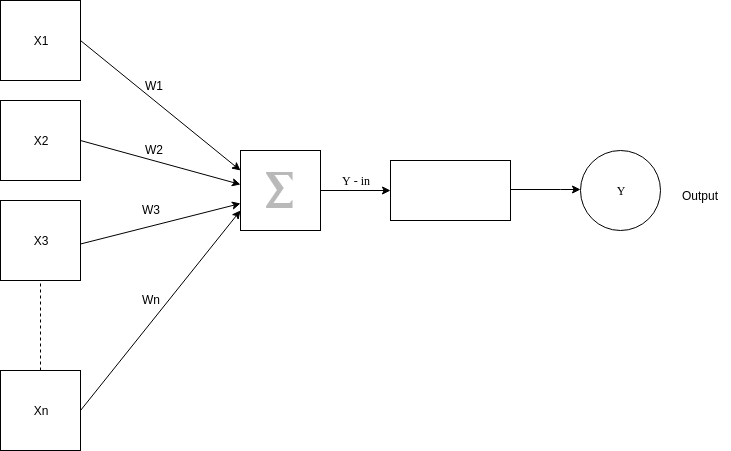
\includegraphics[height=7cm]{Pictures/ann_model.png}
%\caption{}
%\label{fig5}
%\end{figure}

For the above general model of artificial neural network, the net input can be calculated as follows −

\[Y_{in} = x_{1}*w_{1} + x_{2}*w_{2} + x_{3}*w_{3} + .....+ X_{n}*w_{n}\]

i.e., net input

\[y_{in} = \sum_{i}^{n} x_{i}*w_{i}\]

The output can be calculated by applying the activation function over the net input.
\[Y = F(Y_{in})\]
Output = function (net input calculated)

Processing of ANN depends upon the following three building blocks −

\begin{itemize}
\item Network Topology
\item Adjustments of Weights or Learning
\item Activation Functions

\end{itemize}

\section{NETWORK TOPOLOGY}
A network topology is the arrangement of a network along with its nodes and connecting lines. According to the topology, ANN can be classified as the following kinds −

\subsection{Feedforword Network}
It is a non-recurrent network having processing units/nodes in layers and all the nodes in a layer are connected with the nodes of the previous layers. The connection has different weights upon them. There is no feedback loop means the signal can only flow in one direction, from input to output. It may be divided into the following two types −

\begin{itemize}
\item \textbf{Single layer feedforward network: } The concept is of feedforward ANN having only one weighted layer. In other words, we can say the input layer is fully connected to the output layer.

\end{itemize}

%\begin{figure}[htbp]
%\centering
%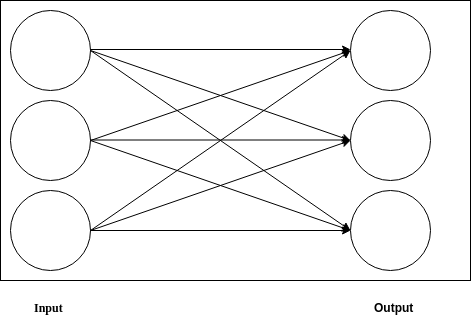
\includegraphics[height=7cm]{Pictures/Single layer feedforward network.png}
%\caption{}
%\label{fig5}
%\end{figure}

\begin{itemize}
\item \textbf{Multi layer feedforward network: } The concept is of feedforward ANN having more than one weighted layer. As this network has one or more layers between the input and the output layer, it is called hidden layers.


\end{itemize}

%\begin{figure}[htbp]
%\centering
%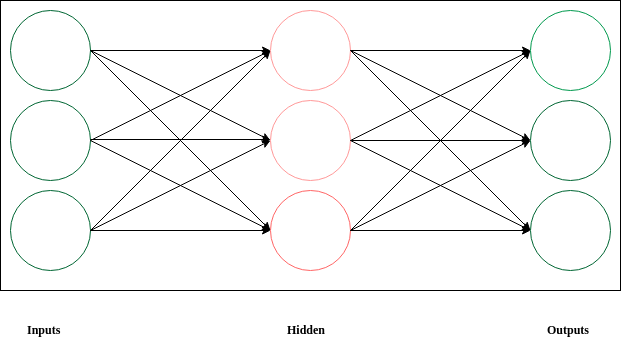
\includegraphics[height=7cm]{Pictures/Multilayer feedforward network.png}
%\caption{}
%\label{fig5}
%\end{figure}

\subsection{Feedback Network}
As the name suggests, a feedback network has feedback paths, which means the signal can flow in both directions using loops. This makes it a non-linear dynamic system, which changes continuously until it reaches a state of equilibrium. It may be divided into the following types −

\begin{itemize}
\item \textbf{Recurrent networks} They are feedback networks with closed loops. Following are the two types of recurrent networks.

\item \textbf{Fully recurrent network} It is the simplest neural network architecture because all nodes are connected to all other nodes and each node works as both input and output.

%\begin{figure}[htbp]
%\centering
%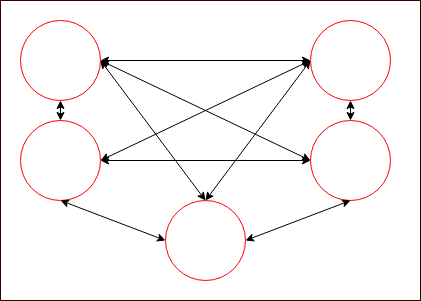
\includegraphics[height=7cm]{Pictures/Fully recurrent network.png}
%\caption{}
%\label{fig5}
%\end{figure}

\item \textbf{Jordan network} It is a closed loop network in which the output will go to the input again as feedback as shown in the following diagram.


%\begin{figure}[htbp]
%\centering
%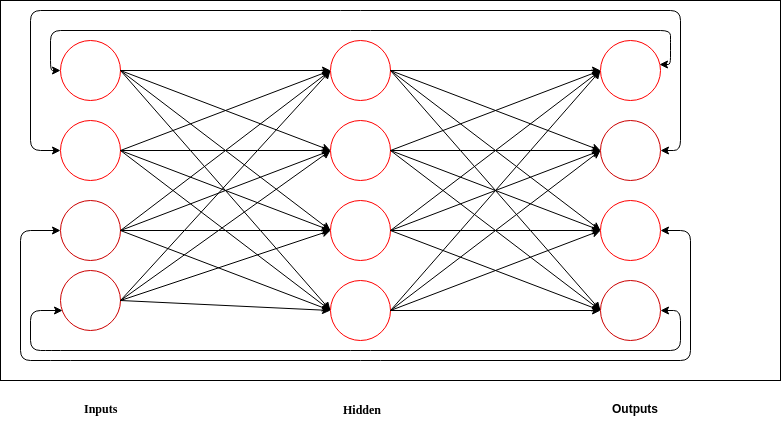
\includegraphics[height=7cm]{Pictures/Jordan network.png}
%\caption{}
%\label{fig5}
%\end{figure}

\end{itemize}

%\begin{table}[htbp]
%\resizebox{1.1\textwidth}{!}{
%\begin{tabular}{|l|l|l|}
%\hline
%Criteria & BNN & ANN \\ \hline
%Processing & Massively parallel, Slow but superior than ANN & Massively Parallel, Fast but inferior than BNN \\ \hline
% &  &  \\ \hline
% &  &  \\ \hline
% &  &  \\ \hline
% &  &  \\ \hline
%\end{tabular}}
%\end{table}


\section{Learning}
The type of learning we will discuss is commonly called supervised learning or error correction learning. The algorithm that we have used to do this is called Back Propagation of Error signals or in short Backprop. Every iteration of the algorith consists of two pases: 

\subsection{Forward Pass: }
Forward pass every perceptron calculates the weighted linear combination of all its inputs and applies to the result of this summing junction an activation function. The result of the activation function provides the perceptron of its output value.

\subsection{Backward Pass: }
 At the output layer of the network we calculate the error with respect to the desired output value for a certain pattern. This error is propagated backwards through the network enforcing a correction on the weights of all connections in the network. This technique is based on the observation that all perceptrons in the network have a shared  responsibility for the error that has been calculated at the output layer.


%\begin{figure}[]
%\centering
%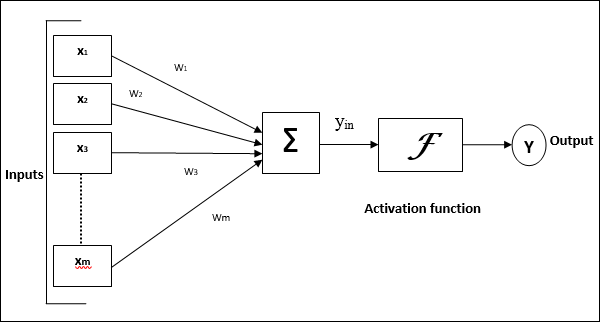
\includegraphics[height=7cm]{Pictures/temp.png}
%\caption{Splitting of the input space (X1 x X2) by M5' model tree algorithm}
%\label{fig5}
%\end{figure}

%\begin{figure}[]
%\centering
%\includegraphics[height=7cm]{Pictures/Neuron3.png}
%\caption{Splitting of the input space (X1 x X2) by %M5' model tree algorithm}
%\label{fig5}
%\end{figure}

%\begin{figure}[]
%\centering
%\includegraphics[height=7cm]{Pictures/neural-%network.png}
%\caption{Splitting of the input space (X1 x X2) by %M5' model tree algorithm}
%\label{fig5}
%\end{figure}


\end{document}


%\input{Chapters/Chapter4} 
%\input{Chapters/Chapter5} 
%\input{Chapters/Chapter6} 
%\input{Chapters/Chapter7} 

%----------------------------------------------------------------------------------------
%	THESIS CONTENT - APPENDICES
%----------------------------------------------------------------------------------------

\addtocontents{toc}{\vspace{2em}} % Add a gap in the Contents, for aesthetics

\appendix % Cue to tell LaTeX that the following 'chapters' are Appendices

% Include the appendices of the thesis as separate files from the Appendices folder
% Uncomment the lines as you write the Appendices

% Appendix Template

\chapter{Appendix A} % Main appendix title

\label{AppendixX} % Change X to a consecutive letter; for referencing this appendix elsewhere, use \ref{AppendixX}

\lhead{Appendix X. \emph{Appendix Title Here}} % Change X to a consecutive letter; this is for the header on each page - perhaps a shortened title

Write your Appendix content here.

%\input{Appendices/AppendixB}
%\input{Appendices/AppendixC}

\addtocontents{toc}{} % Add a gap in the Contents, for aesthetics

\backmatter

%----------------------------------------------------------------------------------------
%	BIBLIOGRAPHY
%----------------------------------------------------------------------------------------
%\nocite{*}
\label{Bibliography}

\lhead{\emph{Bibliography}} % Change the page header to say "Bibliography"

\bibliographystyle{apalike} % Use the "custom" BibTeX style for formatting the Bibliography

\bibliography{Bibliography} % The references (bibliography) information are stored in the file named "Bibliography.bib"

\end{document}  
